% appendix/questions/questions.tex
% mainfile: ../../perfbook.tex
% SPDX-License-Identifier: CC-BY-SA-3.0

\QuickQuizChapter{cha:app:Important Questions}{Important Questions}{qqzquestions}
%
\Epigraph{Ask me no questions, and I'll tell you no fibs.}
	 {\emph{``She Stoops to Conquer'', Oliver Goldsmith}}

The following sections discuss some important questions relating to
SMP programming.
Each section also shows how to avoid worrying about
the corresponding question, which can be extremely important if
your goal is to simply get your SMP code working as quickly and
painlessly as possible---which is an excellent goal, by the way!

Although the answers to these questions are often less
intuitive than they would be in a single-threaded setting,
with a bit of work, they are not that difficult to understand.
If you managed to master recursion, there is nothing here that should
pose an overwhelming challenge.

% @@@ roadmap...

% @@@ doesn't parallel automatically make things faster? (locked increment)
% @@@ doesn't getting rid of locks get rid of all these problems? (atomic inc)
% @@@ doesn't NBS take care of all these problems? (cite IPDPS paper)
% @@@ why isn't more software correct?

% appendix/questions/after.tex
% mainfile: ../../perfbook.tex
% SPDX-License-Identifier: CC-BY-SA-3.0

\section{What Does ``After'' Mean?}
\label{sec:app:questions:What Does ``After'' Mean?}

``After'' is an intuitive, but surprisingly difficult concept.
An important non-intuitive issue is that code can be delayed at
any point for any amount of time.
Consider a producing and a consuming thread that communicate using
a global struct with a timestamp ``t'' and integer fields ``a'', ``b'',
and ``c''.
The producer loops recording the current time
(in seconds since 1970 in decimal),
then updating the values of ``a'', ``b'', and ``c'',
as shown in \cref{lst:app:questions:After Producer Function}.
The consumer code loops, also recording the current time, but also
copying the producer's timestamp along with the fields ``a'',
``b'', and ``c'', as shown in
\cref{lst:app:questions:After Consumer Function}.
At the end of the run, the consumer outputs a list of anomalous recordings,
e.g., where time has appeared to go backwards.

\begin{listing}
\input{CodeSamples/api-pthreads/QAfter/time@producer.fcv}
\caption{``After'' Producer Function}
\label{lst:app:questions:After Producer Function}
\end{listing}

\begin{listing}
\ebresizeverb{.96}{\input{CodeSamples/api-pthreads/QAfter/time@consumer.fcv}}
\caption{``After'' Consumer Function}
\label{lst:app:questions:After Consumer Function}
\end{listing}

\QuickQuiz{
	What SMP coding errors can you see in these examples?
	See \path{time.c} for full code.
}\QuickQuizAnswer{
	Here are errors you might have found:

	\begin{enumerate}
	\item	Missing barrier() or volatile on tight loops.
	\item	Missing memory barriers on update side.
	\item	Lack of synchronization between producer and consumer.
	\end{enumerate}
}\QuickQuizEnd

One might intuitively expect that the difference between the producer
and consumer timestamps would be quite small, as it should not take
much time for the producer to record the timestamps or the values.
An excerpt of some sample output on a dual-core 1\,GHz x86 is shown in
\cref{tab:app:questions:After Program Sample Output}.
Here, the ``seq'' column is the number of times through the loop,
the ``time'' column is the time of the anomaly in seconds, the ``delta''
column is the number of seconds the consumer's timestamp follows that
of the producer (where a negative value indicates that the consumer
has collected its timestamp before the producer did), and the
columns labelled ``a'', ``b'', and ``c'' show the amount that these
variables increased since the prior snapshot collected by the consumer.

\begin{table}
\rowcolors{1}{}{lightgray}
\renewcommand*{\arraystretch}{1.2}
\sisetup{group-digits=false}
\centering
\scriptsize
\begin{tabular}{rS[table-format=7.6]rS[table-format=3.0]S[table-format=3.0]S[table-format=3.0]}
\toprule
seq    & \multicolumn{1}{c}{time (seconds)} & delta~  &  a &  b &  c \\
\midrule
17563: & 1152396.251585 & ($-16.928$) & 27 & 27 & 27 \\
18004: & 1152396.252581 & ($-12.875$) & 24 & 24 & 24 \\
18163: & 1152396.252955 & ($-19.073$) & 18 & 18 & 18 \\
18765: & 1152396.254449 & ($-148.773$) & 216 & 216 & 216 \\
19863: & 1152396.256960 & ($-6.914$) & 18 & 18 & 18 \\
21644: & 1152396.260959 & ($-5.960$) & 18 & 18 & 18 \\
23408: & 1152396.264957 & ($-20.027$) & 15 & 15 & 15 \\
\bottomrule
\end{tabular}
\caption{``After'' Program Sample Output}
\label{tab:app:questions:After Program Sample Output}
\end{table}

Why is time going backwards?
The number in parentheses is the difference in microseconds, with
a large number exceeding 10 microseconds, and one exceeding even
100 microseconds!
Please note that this CPU can potentially execute more than 100,000
instructions in that time.

\begin{fcvref}[ln:api-pthreads:QAfter:time]
One possible reason is given by the following sequence of events:
\begin{enumerate}
\item	Consumer obtains timestamp
	(\cref{lst:app:questions:After Consumer Function},
	\clnref{consumer:tod}).
\item	Consumer is preempted.
\item	An arbitrary amount of time passes.
\item	Producer obtains timestamp
	(\cref{lst:app:questions:After Producer Function},
	\clnref{producer:tod}).
\item	Consumer starts running again, and picks up the producer's
	timestamp
	(\cref{lst:app:questions:After Consumer Function},
	\clnref{consumer:prodtod}).
\end{enumerate}

In this scenario, the producer's timestamp might be an arbitrary
amount of time after the consumer's timestamp.

How do you avoid agonizing over the meaning of ``after'' in your
SMP code?

Simply use SMP primitives as designed.

In this example, the easiest fix is to use locking, for example,
acquire a lock in the producer before \clnref{producer:tod} in
\cref{lst:app:questions:After Producer Function} and in
the consumer before \clnref{consumer:tod} in
\cref{lst:app:questions:After Consumer Function}.
This lock must also be released after \clnref{producer:upd:c} in
\cref{lst:app:questions:After Producer Function} and
after \clnref{consumer:upd:c} in
\cref{lst:app:questions:After Consumer Function}.
These locks cause the code segments in
\clnrefrange{producer:tod}{producer:upd:c} of
\cref{lst:app:questions:After Producer Function} and in
\clnrefrange{consumer:tod}{consumer:upd:c} of
\cref{lst:app:questions:After Consumer Function} to {\em exclude}
each other, in other words, to run atomically with respect to each other.
This is represented in
\cref{fig:app:questions:Effect of Locking on Snapshot Collection}:
The locking prevents any of the boxes of code from overlapping in time, so
that the consumer's timestamp must be collected after the prior
producer's timestamp.
The segments of code in each box in this figure are termed
``critical sections''; only one such critical section may be executing
at a given time.
\end{fcvref}

\begin{figure}
\centering
\includegraphics{appendix/questions/after-snapshot}
\caption{Effect of Locking on Snapshot Collection}
\label{fig:app:questions:Effect of Locking on Snapshot Collection}
\end{figure}

This addition of locking results in output as shown in
\cref{fig:app:questions:Locked After Program Sample Output}.
Here there are no instances of time going backwards, instead,
there are only cases with more than 1,000 counts difference between
consecutive reads by the consumer.

\begin{table}
\renewcommand*{\arraystretch}{1.2}
\sisetup{group-digits=false}
\centering
\scriptsize
\begin{tabular}{rS[table-format=7.6]rS[table-format=4.0]S[table-format=4.0]S[table-format=4.0]}
\toprule
seq    & \multicolumn{1}{c}{time (seconds)} & delta~  &  a &  b &  c \\
\midrule
58597:  & 1156521.556296 & ($3.815$) & 1485 & 1485 & 1485 \\
403927: & 1156523.446636 & ($2.146$) & 2583 & 2583 & 2583 \\
\bottomrule
\end{tabular}
\caption{Locked ``After'' Program Sample Output}
\label{fig:app:questions:Locked After Program Sample Output}
\end{table}

\QuickQuiz{
	How could there be such a large gap between successive
	consumer reads?
	See \path{timelocked.c} for full code.
}\QuickQuizAnswer{
	Here are a few reasons for such gaps:

	\begin{enumerate}
	\item	The consumer might be preempted for long time periods.
	\item	A long-running interrupt might delay the consumer.
	\item	Cache misses might delay the consumer.
	\item	The producer might also be running on a faster CPU than is the
		consumer (for example, one of the CPUs might have had to
		decrease its
		clock frequency due to heat-dissipation or power-consumption
		constraints).
	\end{enumerate}
}\QuickQuizEnd

In summary, if you acquire an \IXh{exclusive}{lock}, you {\em know} that
anything you do while holding that lock will appear to happen after
anything done by any prior holder of that lock, at least give or
take \IXacrl{tle}
(see \cref{sec:future:Semantic Differences}).
No need to worry about which CPU did or did not execute a memory
barrier, no need to worry about the CPU or compiler reordering
operations---life is simple.
Of course, the fact that this locking prevents these two pieces of
code from running concurrently might limit the program's ability
to gain increased performance on multiprocessors, possibly resulting
in a ``safe but slow'' situation.
\Cref{cha:Partitioning and Synchronization Design} describes ways of
gaining performance and scalability in many situations.

In short, in many parallel programs, the really important definition
of ``after'' is ordering of operations, which is covered in dazzling
detail in
\cref{chp:Advanced Synchronization: Memory Ordering}.

However, in most cases, if you find yourself worrying about what happens
before or after a given piece of code, you should take this as a hint to
make better use of the standard primitives.
Let these primitives do the worrying for you.

% appendix/questions/concurrentparallel.tex
% mainfile: ../../perfbook.tex
% SPDX-License-Identifier: CC-BY-SA-3.0

\section{What is the Difference Between ``Concurrent'' and ``Parallel''?}
\label{sec:app:questions:What is the Difference Between ``Concurrent'' and ``Parallel''?}

From a classic computing perspective, ``concurrent'' and ``parallel''
are clearly synonyms.
However, this has not stopped many people from drawing distinctions
between the two, and it turns out that these distinctions can be
understood from a couple of different perspectives.

The first perspective treats ``parallel'' as an abbreviation for
``data parallel'', and treats ``concurrent'' as pretty much everything
else.
From this perspective, in parallel computing, each partition of the
overall problem can proceed completely independently, with no
communication with other partitions.
In this case, little or no coordination among partitions is required.
In contrast, concurrent computing might well have tight interdependencies,
in the form of contended locks, transactions, or other synchronization
mechanisms.

\QuickQuiz{
	Suppose a portion of a program uses RCU read-side primitives
	as its only synchronization mechanism.
	Is this parallelism or concurrency?
}\QuickQuizAnswer{
	Yes.
}\QuickQuizEnd

This of course begs the question of why such a distinction matters,
which brings us to the second perspective, that of the underlying scheduler.
Schedulers come in a wide range of complexities and capabilities, and
as a rough rule of thumb, the more tightly and irregularly a set of
parallel processes communicate, the higher the level of sophistication
required from the scheduler.
As such, parallel computing's avoidance of interdependencies means that
parallel-computing programs run well on the least-capable schedulers.
In fact, a pure parallel-computing program can run successfully after
being arbitrarily subdivided and interleaved onto a uniprocessor.\footnote{
	Yes, this does mean that data-parallel-computing programs are
	best-suited for sequential execution.
	Why did you ask?}
In contrast, concurrent-computing programs might well require extreme
subtlety on the part of the scheduler.

One could argue that we should simply demand a reasonable level of
competence from the scheduler, so that we could simply ignore any
distinctions between parallelism and concurrency.
Although this is often a good strategy,
there are important situations where efficiency,
performance, and scalability concerns sharply limit the level
of competence that the scheduler can reasonably offer.
One important example is when the scheduler is implemented in
hardware, as it often is in SIMD units or GPGPUs.
Another example is a workload where the units of work are quite
short, so that even a software-based scheduler must make hard choices
between subtlety on the one hand and efficiency on the other.

Now, this second perspective can be thought of as making the workload
match the available scheduler, with parallel workloads able to
use simple schedulers and concurrent workloads requiring
sophisticated schedulers.

Unfortunately, this perspective does not always align with the
dependency-based distinction put forth by the first perspective.
For example, a highly interdependent lock-based workload
with one thread per CPU can make do with a trivial scheduler
because no scheduler decisions are required.
In fact, some workloads of this type can even be run one after another
on a sequential machine.
Therefore, such a workload would be labeled ``concurrent'' by the first
perspective and ``parallel'' by many taking the second perspective.

\QuickQuiz{
	In what part of the second (scheduler-based) perspective would
	the lock-based single-thread-per-CPU workload be considered
	``concurrent''?
}\QuickQuizAnswer{
	The people who would like to arbitrarily subdivide and interleave
	the workload.
	Of course, an arbitrary subdivision might end up separating
	a lock acquisition from the corresponding lock release, which
	would prevent any other thread from acquiring that lock.
	If the locks were pure spinlocks, this could even result in
	deadlock.
}\QuickQuizEnd

Which is just fine.
No rule that humankind writes carries any weight against the objective
universe, not even rules dividing multiprocessor programs into categories
such as ``concurrent'' and ``parallel''.

This categorization failure does not mean such rules are useless,
but rather that you should take on a suitably skeptical frame of mind when
attempting to apply them to new situations.
As always, use such rules where they apply and ignore them otherwise.

In fact, it is likely that new categories will arise in addition
to parallel, concurrent, map-reduce, task-based, and so on.
Some will stand the test of time, but good luck guessing which!

% appendix/questions/time.tex
% mainfile: ../../perfbook.tex
% SPDX-License-Identifier: CC-BY-SA-3.0

\section{What Time Is It?}
\label{sec:app:questions:What Time Is It?}

\begin{figure}
\centering
\resizebox{2.6in}{!}{\includegraphics{cartoons/r-2014-What-time-is-it}}
\caption{What Time Is It?}
\ContributedBy{Figure}{fig:app:questions:What Time Is It?}{Melissa Broussard}
\end{figure}

A key issue with timekeeping on multicore computer systems is illustrated
by \cref{fig:app:questions:What Time Is It?}.
One problem is that it takes time to read out the time.
An instruction might read from a hardware clock, and might
have to go off-core (or worse yet, off-socket) to complete
this read operation.
It might also be necessary to do some computation on the value read out,
for example, to convert it to the desired format, to apply network time
protocol (NTP) adjustments, and so on.
So does the time eventually returned correspond to the beginning of
the resulting time interval, the end, or somewhere in between?

Worse yet, the thread reading the time might be interrupted or preempted.
Furthermore, there will likely be some computation between reading out
the time and the actual use of the time that has been read out.
Both of these possibilities further extend the interval of uncertainty.

One approach is to read the time twice, and take the arithmetic mean
of the two readings, perhaps one on each side of the operation being
timestamped.
The difference between the two readings is then a measure of uncertainty
of the time at which the intervening operation occurred.

Of course, in many cases, the exact time is not necessary.
For example, when printing the time for the benefit of a human user,
we can rely on slow human reflexes to render internal hardware and
software delays irrelevant.
Similarly, if a server needs to timestamp the response to a client, any
time between the reception of the request and the transmission of the
response will do equally well.

There is an old saying that those who have but one clock always
know the time, but those who have several clocks can never be sure.
And there was a time when the typical low-end computer's sole
software-visible clock was its program counter, but those days are
long gone.
This is not a bad thing, considering that on modern computer systems,
the program counter is a truly horrible
clock~\cite{PeterOkech2009InherentRandomness}.

In addition, different clocks provide different tradeoffs of performance,
accuracy, precision, and ordering.
For example, in the Linux kernel, the \co{jiffies} counter\footnote{
	The \co{jiffies} variable is a location in normal memory that
	is incremented by software in response to events such as the
	scheduling-clock interrupt.}
provides high-speed access to a course-grained counter (at best
one-millisecond accuracy and precision) that imposes very little ordering
on either the compiler or the hardware.
In contrast, the x86 HPET hardware provides an accurate and
precise clock, but at the price of slow access.
The x86 time-stamp counter (TSC) has a checkered past, but is more
recently held out as providing a good combination of precision, accuracy,
and performance.
Unfortunately, for all of these counters, ordering against all effects
of prior and subsequent code requires expensive memory-barrier instructions.
And this expense appears to be an unavoidable consequence of the
complex superscalar nature of modern computer systems.

\begin{figure}
\centering
\resizebox{3in}{!}{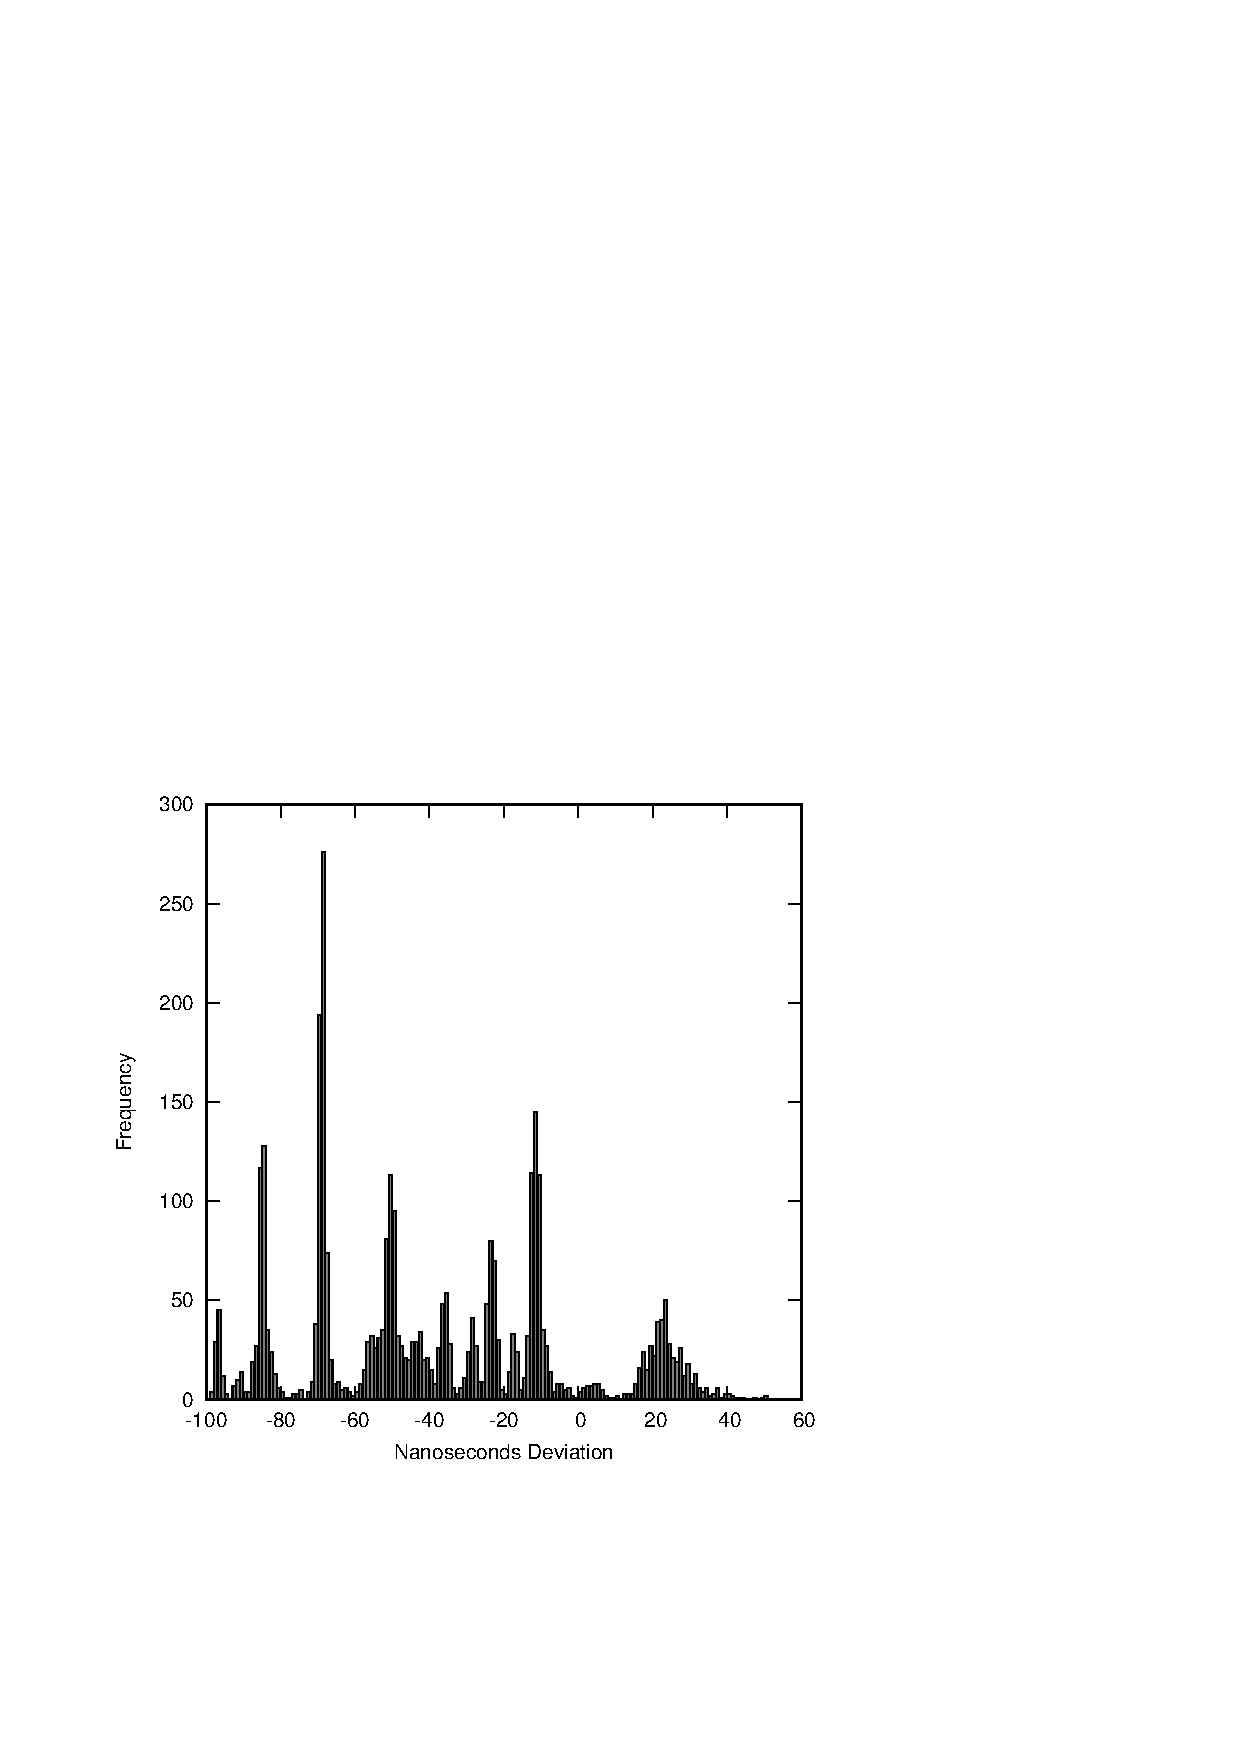
\includegraphics{CodeSamples/api-pthreads/QAfter/timeskewhist}}
\caption{\tco{clock_gettime(CLOCK_REALTIME)} Deviation From Immediately Preceding \tco{clock_gettime(CLOCK_MONOTONIC)}}
\label{fig:app:questions:clock-gettime(CLOCK-REALTIME) Deviation From Immediately Preceding clock-gettime(CLOCK-MONOTONIC)}
\end{figure}

In addition, each clock source provides its own timebase.
\Cref{fig:app:questions:clock-gettime(CLOCK-REALTIME) Deviation From Immediately Preceding clock-gettime(CLOCK-MONOTONIC)}
shows a histogram of the value returned by a call to
\co{clock_gettime(CLOCK_MONOTONIC)} subtracted from that returned by an
immediately following \co{clock_gettime(CLOCK_REALTIME)}
(\path{timeskew.c}).
Because some time passes between these two function calls, it is no
surprise that there are positive deviations, but the negative deviations
should give us some pause.
Nevertheless, such deviations are possible, if for no other reason than
the machinations of network time protocol (NTP).

Worse yet, identical clocksources on different systems
are not necessarily compatible with that of another.
For example, the \co{jiffies} counters on a pair of systems very likely
started counting at different times, and worse yet might well be counting
at different rates.
This brings up the topic of synchronizing a given system's counters
with some real-world notion of time such as the aforementioned NTP,
but that topic is beyond the scope of this book.

In short, time is a slippery topic that causes untold confusion to
parallel programmers and to their code.

% appendix/questions/ordering.tex
% mainfile: ../../perfbook.tex
% SPDX-License-Identifier: CC-BY-SA-3.0

\section{How Much Ordering Is Needed?}
\label{sec:app:questions:How Much Ordering Is Needed?}

Perhaps you have carefully constructed a strongly ordered concurrent
system, only to find that it neither performs nor scales well.
Or perhaps you threw caution to the wind, only to find that your
brilliantly fast and scalable software is also unreliable.
Is there a happy medium with both robust reliability on the one
hand and powerful performance augmented by scintellating scalability on
the other?

The answer, as is so often the case, is ``it depends''.

One approach is to construct a strongly ordered system, then examine
its performance and scalablity.
If these suffice, the system is good and sufficient, and no more need
be done.
Otherwise, undertake careful analysis
(see \cref{sec:debugging:Performance Estimation})
and attack each bottleneck until the system's performance is good and
sufficient.

This approach can work very well, especially in contrast to the
all-too-common approach of optimizing random components of the system
in the hope of achieving significant system-wide benefits.
However, starting with strong ordering can also be quite wasteful,
given that weakening ordering of the system's bottleneck can require
that large portions of the rest of the system be redesigned and
rewritten to accommodate the weakening.
Worse yet, eliminating one bottleneck often exposes another, which
in turn needs to be weakened and which in turn can result in wholesale
redesigns and rewrites of other parts of the system.
Perhaps even worse is the approach, also common, of starting with a
fast but unreliable system and then playing whack-a-mole with an endless
succession of concurrency bugs, though in the latter case,
\cref{chp:Validation,chp:Formal Verification}
are always there for you.

It would be better to have design-time tools to determine which portions
of the system could use weak ordering, and at the same time, which
portions actually benefit from weak ordering.
These tasks are taken up by the following sections.

\subsection{Where is the Defining Data?}
\label{sec:app:questions:Where is the Defining Data?}

One way to do this is to keep firmly in mind that the region of
consistency engendered by strong ordering cannot extend out past the
boundaries of the system.\footnote{
	Which might well be a distributed system.}
Portions of the system whose role is to track the state of the outside
world can usually feature weak ordering, given that speed-of-light delays
will force the within-system state to lag that of the outside world.
There is often no point in incurring large overheads to force a consistent
view of data that is inherently out of date.
In these cases, the methods of \cref{chp:Deferred Processing} can be
quite helpful, as can some of the data structures described in
\cref{chp:Data Structures}.

Nevertheless, it is wise to adopt some meaningful semantics that are
visible to those accessing the data, for example, a given function's
return value might be:

\begin{enumerate}
\item	Some value between the conceptual value at the time of the call
	to the function and the conceptual value at the time of the
	return from that function.
	For example, see the statistical counters discussed in
	\cref{sec:count:Statistical Counters}, keeping in mind that such
	counters are normally monotonic, at least between consecutive
	overflows.
\item	The actual value at some time between the call to and the return
	from that function.
	For example, see the single-variable atomic counter shown in
	\cref{lst:count:Just Count Atomically!}.
\item	If the values used by that function remain unchanged during the
	time between that function's call and return, the expected
	value, otherwise some approximation to the expected value.
	Precise specification of the bounds on the approximation can
	be quite challenging.
	For example, consider a function combining values from
	different elements of an RCU-protected linked data structure,
	as described in \cref{sec:datastruct:Read-Mostly Data Structures}.
\end{enumerate}

Weaker ordering usually implies weaker semantics, and you should be
able to give some sort of promise to your users as to how this weakening
affects them.
At the same time, unless the caller holds a lock across both the
function call and the use of any values computed by that function,
even fully ordered implementations normally cannot do any better
than the semantics given by the options above.

\QuickQuiz{
	But if fully ordered implementations cannot offer stronger
	guarantees that the better performing and more scalable weakly
	ordered imptementations, why bother with full ordering?
}\QuickQuizAnswer{
	Because strongly ordered implementations are sometimes
	able to provide greater consistency among sets of calls to
	functions accessing a given data structure.
	For example, compare the atomic counter of
	\cref{lst:count:Just Count Atomically!}
	to the statistical counter of
	\cref{sec:count:Statistical Counters}.
	Suppose that one thread is adding the value~3 and another is
	adding the value~5, while two other threads are concurrently
	reading the counter's value.
	With atomic counters, it is not possible for one of the readers
	to obtain the value~3 while the other obtains the value~5.
	With statistical counters, this outcome really can happen.
	In fact, in some computing environments, this outcome can happen
	even on relatively strongly ordered hardware such as x86.

	Therefore, if your user happen to need this admittedly
	unusual level of consistency, you should avoid weakly ordered
	statistical counters.
}\QuickQuizEnd

Some might argue that useful computing deals only with the outside world,
and therefore that all computing can use weak ordering.
Such arguments are incorrect.
For example, the value of your bank account is defined within your
bank's computers, and people often prefer exact computations involving
their account balances, especially those who might suspect that any such
approximations would be in the bank's favor.

In short, although data tracking external state can be an attractive
candidate for weakly ordered access, please think carefully about
exactly what is being tracked and what is doing the tracking.

\subsection{Consistent Data Used Consistently?}
\label{sec:app:questions:Consistent Data Used Consistently?}

Another hint that weakening is safe can appear in the guise of data
that is computed while holding a lock, but then used after the lock
is released.
The computed result clearly becomes at best an approximation as soon as
the lock is released, which suggests computing an approximate result
in the first place, possibly permitting use of weaker ordering.
To this end, \cref{chp:Counting} covers numerous approximate methods
for counting.

Great care is required, however.
Is the use of data following lock release a hint that weak-ordering
optimizations might be helpful?
Or is instead a bug in which the lock was released too soon?

\subsection{Is the Problem Partitionable?}
\label{sec:app:questions:Is the Problem Partitionable?}

Suppose that the system holds the defining instance of the data,
or that using a computed value past lock release proved to be a bug.
What then?

One approach is to partition the system, as discussed in
\cref{cha:Partitioning and Synchronization Design}.
Partititioning can provide excellent scalability and in its more
extreme form, per-CPU performance rivaling that of a sequential program,
as discussed in \cref{chp:Data Ownership}.
Partial partitioning is often mediated by locking, which is the subject of
\cref{chp:Locking}.

\subsection{None of the Above?}
\label{sec:app:questions:None of the Above?}

The previous sections described the easier ways to gain performance
and scalability, sometimes using weaker ordering and sometimes not.
But the plain fact is that multicore systems are under no compunction
to make life easy.
But perhaps the advanced topics covered in
\cref{sec:advsync:Advanced Synchronization,%
chp:Advanced Synchronization: Memory Ordering}
will prove helpful.

But please proceed with care, as it is all too easy to destabilize
your codebase optimizing non-bottlenecks.
Once again, \cref{sec:debugging:Performance Estimation} can help.
It might also be worth your time to review other portions of this
book, as it contains much information on handling a number of tricky
situations.


\QuickQuizAnswersChp{qqzquestions}
